\documentclass[11pt]{report}
\usepackage[utf8]{inputenc}
\usepackage[T1]{fontenc}
\usepackage{amsmath,amssymb,amsfonts}
\usepackage{booktabs}
\usepackage{geometry}
\geometry{letterpaper,margin=1in}
\usepackage{microtype}
\usepackage[table]{xcolor}
\usepackage{tikz}
\usetikzlibrary{shapes,arrows,positioning,calc,decorations.pathmorphing,backgrounds}
\usepackage{float}
\usepackage{mdframed}
\usepackage{hyperref}
\hypersetup{
    colorlinks=true,
    linkcolor=teal,
    citecolor=teal,
    urlcolor=teal
}

\newmdenv[
  linecolor=black,
  linewidth=1pt,
  innertopmargin=10pt,
  innerbottommargin=10pt,
  innerrightmargin=12pt,
  innerleftmargin=12pt,
  backgroundcolor=gray!5
]{blackboard}

\title{\Huge\textbf{The Feynman Lectures on Social Physics}\\
\Large The Classical Mechanics of Human Risk, Boundaries, and Sacred Trust}
\author{\textbf{Adam Matthew Steinberger}}
\date{October 2026}

\begin{document}

\maketitle

\tableofcontents
\newpage

\chapter*{Preface}
\addcontentsline{toc}{chapter}{Preface}

Most people think philosophy is a collection of academic figures arguing over undefined terms, using complex vocabularies to conceal ambiguity.

Interpersonal relationships suffer even more from sentimentality. Cultural adages demand complete openness, universal trust, and the elimination of personal boundaries. That assumption is unscientific and dangerous. If an engineer built an airplane using that thinking, the wings would sheer off before the aircraft cleared the tarmac.

Nature operates independently of human wishes. If you ignore the laws of mechanics, gravity pulls you down to the pavement. If you ignore the mechanics of human nature, such as the reality of fallen self-interest, envy, deceit for ego preservation, gossip, and abandonment under pressure, social and financial ruin follow.

The first principle requires that you refrain from fooling yourself, especially because you are the easiest person to fool. In these lectures, we examine the machinery of human social life: the behavior of trust as an asymmetric capacitor, the function of boundaries as radiation shielding, the ancient social risk formulations of Sirach and Thomas Aquinas, and the objective calculation of interpersonal risk.

\chapter{The First Principle: Realistic Human Nature}

\section{The Office Hours After the Discharge}
The door to 103 Bridge Annex stood half open. Inside, a chalkboard held Feynman diagrams, Maxwell stress tensors, and in the corner, a quote chalked in red: \textit{John 2:24}.

Daniel knocked twice. His shoulders hung low.

``Come in, come in!'' Feynman said, setting down a pair of brass calipers. He held a glass of tea in one hand and a chalk stub in the other. ``Step into the room, Daniel. You are blocking the light. What happened? You look like you caught a high-voltage discharge.''

``I did, Professor,'' Daniel said, sitting down heavily on a wooden folding chair. ``The project with Miller and the student council ended in disaster. I gave them my entire design notebook: every calculation, all the drafts, and my personal notes about department funding vulnerabilities. I trusted them.''

``What did the experiment reveal?'' Feynman asked, leaning forward.

``Miller presented the notebook to Dean Harrison, cut my name off the cover, used my notes about the funding to freeze my lab stipend, and told the council I was unstable and withholding data. Half the department avoids eye contact with me.''

Feynman took a sip of tea. ``Your surprise is the real puzzle.''

Daniel blinked. ``I believed Christians practiced unconditional trust. Love believes all things.''

Feynman set his tea on the desk. ``Look at the primary text. Read John chapter two, verses twenty-three to twenty-five chalked on the board.''

Daniel read aloud:
\begin{quote}
\textit{``Now when he was in Jerusalem at the Passover Feast, many believed in his name when they saw the signs that he was doing. But Jesus on his part did not entrust himself to them, because he knew all people and needed no one to bear witness about man, for he himself knew what was in man.''}
\end{quote}

Feynman paced behind his desk. ``Examine the Greek vocabulary. The crowd believed in Him: \textit{episteusan}. Jesus withheld personal entrustment: \textit{ouk episteuen auton}. The evangelist uses the identical root. The crowd trusted Him, yet Jesus declined to entrust Himself to them. He loved them enough to die for their redemption on the cross. Simultaneously, He protected His schedule, His physical safety, and His private counsels, because He understood the mechanics of human nature.''

``He understood human fallenness,'' Daniel said.

``Precisely. The theologians formulate this as \textit{homo incurvatus in se}, the human person curved inward upon the self. In physics, an engineer calculating the load on an iron beam accounts for microscopic cracks in the lattice. Assuming an iron beam is a flawless crystal leads to structural failure. Human beings have original sin: vanity, fear, cowardice, and self-preservation. Handing Miller an unverified notebook full of personal liabilities was an engineering failure. You handed an ignition source to volatile fuel.''

\begin{figure}[H]
\centering
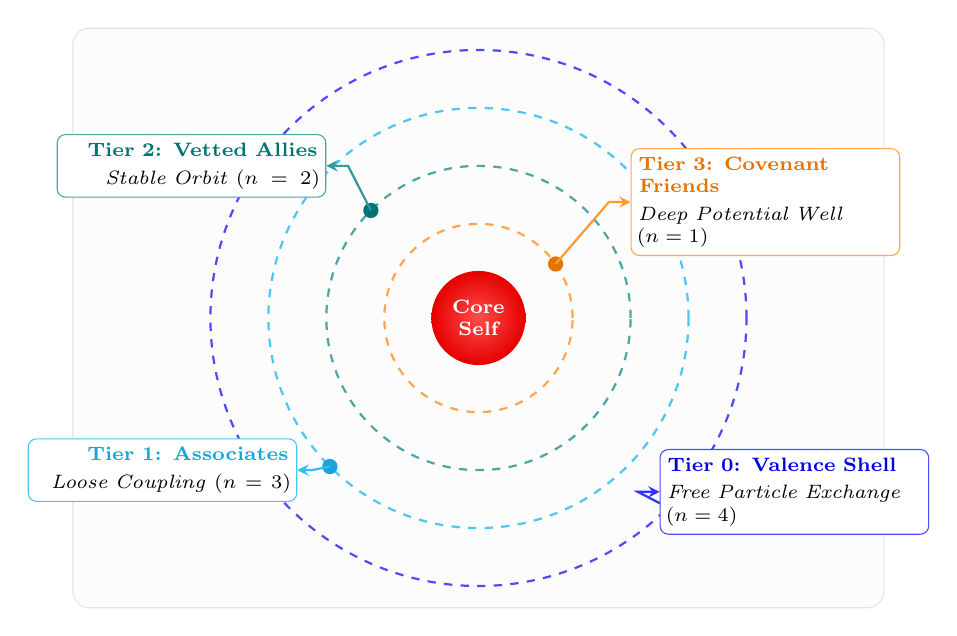
\begin{tikzpicture}[scale=0.92, >=stealth]
  % Bounding box for predictable layout
  \draw[gray!20, fill=gray!2, rounded corners=6pt] (-5.6, -4.0) rectangle (5.6, 4.0);

  % Core Nucleus
  \shade[inner color=red!70, outer color=red!90!black] (0,0) circle (0.65cm);
  \node[font=\bfseries\scriptsize, white, align=center] at (0,0) {Core\\Self};

  % Concentric Orbits (Dashed energy levels)
  \draw[thick, orange!70, dashed] (0,0) circle (1.3cm);
  \draw[thick, teal!70, dashed] (0,0) circle (2.1cm);
  \draw[thick, cyan!70, dashed] (0,0) circle (2.9cm);
  \draw[thick, blue!70, dashed] (0,0) circle (3.7cm);

  % Electron particles on orbits
  \fill[orange!90!black] (35:1.3cm) circle (3pt);
  \fill[teal!90!black] (135:2.1cm) circle (3pt);
  \fill[cyan!90!black] (225:2.9cm) circle (3pt);
  \fill[blue!90!black] (315:3.7cm) circle (3pt);

  % Clean callout cards radiating outwards
  % Tier 3
  \draw[thick, orange!80, ->] (35:1.3cm) -- (1.8, 1.6) -- (2.1, 1.6);
  \node[anchor=west, font=\scriptsize, fill=white, draw=orange!70, rounded corners=3pt, inner sep=3pt, text width=3.2cm, align=left] at (2.1, 1.6) {
    \textbf{\textcolor{orange!90!black}{Tier 3: Covenant Friends}}\\[2pt]
    \textit{Deep Potential Well} ($n=1$)
  };

  % Tier 2
  \draw[thick, teal!80, ->] (135:2.1cm) -- (-1.8, 2.1) -- (-2.1, 2.1);
  \node[anchor=east, font=\scriptsize, fill=white, draw=teal!70, rounded corners=3pt, inner sep=3pt, text width=3.2cm, align=right] at (-2.1, 2.1) {
    \textbf{\textcolor{teal!90!black}{Tier 2: Vetted Allies}}\\[2pt]
    \textit{Stable Orbit} ($n=2$)
  };

  % Tier 1
  \draw[thick, cyan!80, ->] (225:2.9cm) -- (-2.3, -2.1) -- (-2.5, -2.1);
  \node[anchor=east, font=\scriptsize, fill=white, draw=cyan!70, rounded corners=3pt, inner sep=3pt, text width=3.2cm, align=right] at (-2.5, -2.1) {
    \textbf{\textcolor{cyan!90!black}{Tier 1: Associates}}\\[2pt]
    \textit{Loose Coupling} ($n=3$)
  };

  % Tier 0
  \draw[thick, blue!80, ->] (315:3.7cm) -- (2.2, -2.4) -- (2.5, -2.4);
  \node[anchor=west, font=\scriptsize, fill=white, draw=blue!70, rounded corners=3pt, inner sep=3pt, text width=3.2cm, align=left] at (2.5, -2.4) {
    \textbf{\textcolor{blue!90!black}{Tier 0: Valence Shell}}\\[2pt]
    \textit{Free Particle Exchange} ($n=4$)
  };
\end{tikzpicture}
\caption{\textbf{Atomic Orbital Model of Social Physics.} Bound states within deep potential wells require high binding energy, while valence particles exchange freely at the perimeter.}
\label{fig:atomicshell}
\end{figure}

\chapter{The Geometry of the Social Field: Concentric Spheres}

\section{Potential Wells and Boundary Conditions}
Feynman turned to the chalkboard, grabbed an eraser, and cleared a large circle.

``Let us construct a physical model,'' Feynman said, drawing five concentric rings. ``In atomic physics, particles occupy distinct shells. Inner electrons sit tightly bound inside a deep potential well. Valence electrons on the perimeter exchange easily. If an atom allowed every passing particle into its nucleus, immediate fission would destroy the lab.''

\begin{blackboard}
\textbf{The Five Concentric Spheres of Social Interaction:}
\begin{enumerate}
    \item \textbf{Tier 0: Public Wilderness} (Crowds, Strangers, Competitors)
    \item \textbf{Tier 1: Functional Associates} (Colleagues, Lab-mates, Neighbors)
    \item \textbf{Tier 2: Vetted Allies} (Tested Mission Partners, Co-Laborers)
    \item \textbf{Tier 3: The Covenantal Circle} (The Few / ``One in a Thousand'')
    \item \textbf{Tier 4: The Holy of Holies} (God, Lawful Spouse)
\end{enumerate}
\end{blackboard}

\begin{figure}[H]
\centering
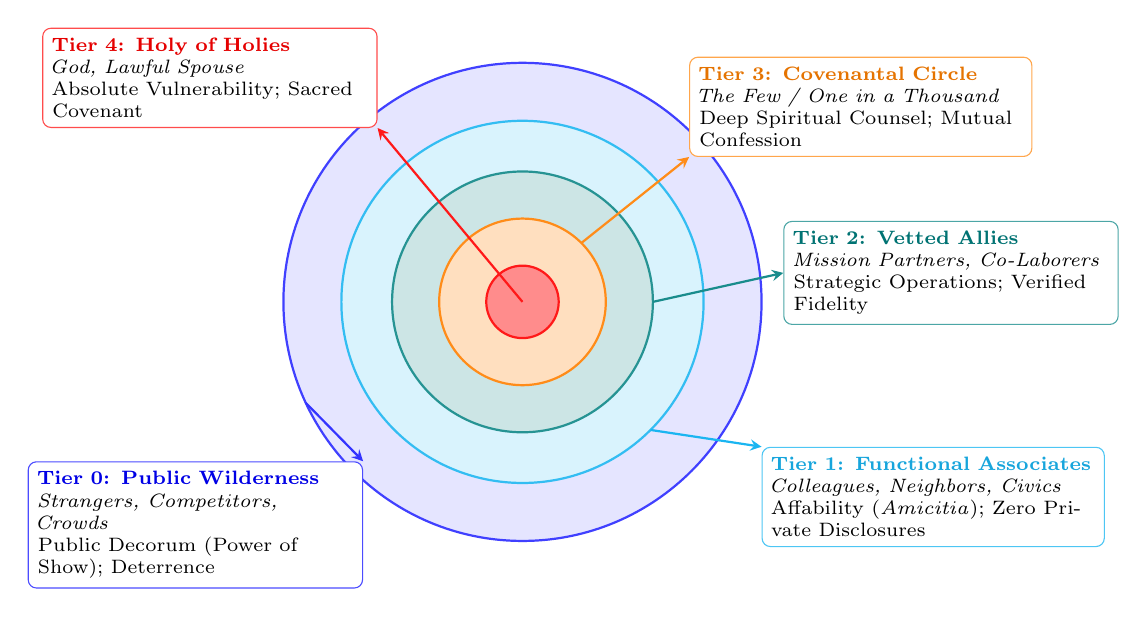
\begin{tikzpicture}[scale=0.92, >=stealth]
  \fill[blue!10] (0,0) circle (3.3cm);
  \fill[cyan!15] (0,0) circle (2.5cm);
  \fill[teal!20] (0,0) circle (1.8cm);
  \fill[orange!25] (0,0) circle (1.15cm);
  \fill[red!45] (0,0) circle (0.5cm);

  \draw[thick, blue!75] (0,0) circle (3.3cm);
  \draw[thick, cyan!80] (0,0) circle (2.5cm);
  \draw[thick, teal!85] (0,0) circle (1.8cm);
  \draw[thick, orange!90] (0,0) circle (1.15cm);
  \draw[thick, red!90] (0,0) circle (0.5cm);

  % Radial pin labels with spacious callout boxes
  \draw[thick, red!90, ->] (0,0) -- (-2.0, 2.4);
  \node[anchor=south east, font=\scriptsize, fill=white, draw=red!70, rounded corners=3pt, inner sep=3.5pt, text width=4.0cm, align=left] at (-2.0, 2.4) {
    \textbf{\textcolor{red!90!black}{Tier 4: Holy of Holies}}\\
    \textit{God, Lawful Spouse}\\
    Absolute Vulnerability; Sacred Covenant
  };

  \draw[thick, orange!90, ->] (45:1.15cm) -- (2.3, 2.0);
  \node[anchor=south west, font=\scriptsize, fill=white, draw=orange!70, rounded corners=3pt, inner sep=3.5pt, text width=4.1cm, align=left] at (2.3, 2.0) {
    \textbf{\textcolor{orange!90!black}{Tier 3: Covenantal Circle}}\\
    \textit{The Few / One in a Thousand}\\
    Deep Spiritual Counsel; Mutual Confession
  };

  \draw[thick, teal!90, ->] (0:1.8cm) -- (3.6, 0.4);
  \node[anchor=west, font=\scriptsize, fill=white, draw=teal!70, rounded corners=3pt, inner sep=3.5pt, text width=4.0cm, align=left] at (3.6, 0.4) {
    \textbf{\textcolor{teal!90!black}{Tier 2: Vetted Allies}}\\
    \textit{Mission Partners, Co-Laborers}\\
    Strategic Operations; Verified Fidelity
  };

  \draw[thick, cyan!90, ->] (315:2.5cm) -- (3.3, -2.0);
  \node[anchor=north west, font=\scriptsize, fill=white, draw=cyan!70, rounded corners=3pt, inner sep=3.5pt, text width=4.1cm, align=left] at (3.3, -2.0) {
    \textbf{\textcolor{cyan!90!black}{Tier 1: Functional Associates}}\\
    \textit{Colleagues, Neighbors, Civics}\\
    Affability (\textit{Amicitia}); Zero Private Disclosures
  };

  \draw[thick, blue!80, ->] (205:3.3cm) -- (-2.2, -2.2);
  \node[anchor=north east, font=\scriptsize, fill=white, draw=blue!70, rounded corners=3pt, inner sep=3.5pt, text width=4.0cm, align=left] at (-2.2, -2.2) {
    \textbf{\textcolor{blue!90!black}{Tier 0: Public Wilderness}}\\
    \textit{Strangers, Competitors, Crowds}\\
    Public Decorum (Power of Show); Deterrence
  };
\end{tikzpicture}
\caption{\textbf{Radial Boundary Field.} Step-wise barriers regulate access and information flow.}
\label{fig:radialfield}
\end{figure}

``Look at historical wisdom,'' Feynman continued, tapping the chalk against the board. ``Jesus ben Sirach wrote a treatise on this topic around 180 B.C. Sirach chapter six, verse six states: \textit{`Let those that are at peace with you be many, but let your advisers be one in a thousand.'} That establishes an exact mathematical ratio: one to one thousand.''

``Tier 1 accommodates hundreds of people,'' Daniel noted.

``Thousands,'' Feynman agreed. ``Civility extends to everyone. You greet people politely, maintain professional decorum, and pay your bills. Thomas Aquinas called this \textit{amicitia}, the virtue of affability. It belongs to justice. You owe every human being civility and respect. Advisers, confidants, and those admitted into the deep potential well remain one in a thousand.''

\chapter{The Asymmetry of Trust: Hysteresis and Circuit Breakers}

\section{Trust Accumulation and Dielectric Breakdown}
``People frequently invert the mathematics of trust,'' Feynman said, drawing a graph on the board with \textit{Time and Verified Testing} on the horizontal axis and \textit{Trust ($T$)} on the vertical axis.

``Charging a high-capacitance capacitor requires time,'' Feynman explained. ``Current enters, and charge accumulates through discrete increments:
\begin{equation}
\Delta T = \sum_{k=1}^n \alpha_k \cdot \mu_k
\end{equation}
You conduct small experiments. You loan a colleague ten dollars; prompt repayment yields $\mu_1 = 1$. You share an innocuous confidence; zero leaks yield $\mu_2 = 1$. Trust accumulates arithmetically across years of verified trials in difficult conditions.''

\begin{figure}[H]
\centering
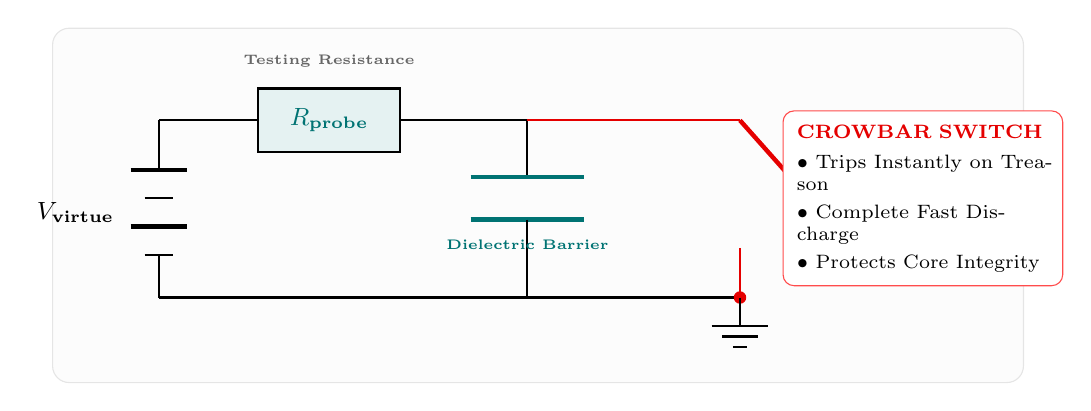
\begin{tikzpicture}[scale=0.90, >=stealth]
  % Boundary Box for aesthetic frame
  \draw[gray!20, fill=gray!2, rounded corners=6pt] (-1.5, -1.2) rectangle (12.2, 3.8);

  % Power source V_virtue
  \draw[thick] (0, 2.5) -- (0, 1.8);
  \draw[ultra thick] (-0.4, 1.8) -- (0.4, 1.8);
  \draw[thick] (-0.2, 1.4) -- (0.2, 1.4);
  \draw[ultra thick] (-0.4, 1.0) -- (0.4, 1.0);
  \draw[thick] (-0.2, 0.6) -- (0.2, 0.6);
  \draw[thick] (0, 0.6) -- (0, 0);
  \node[anchor=east, font=\small\bfseries] at (-0.5, 1.2) {$V_{\text{virtue}}$};

  % Wire to Resistor
  \draw[thick] (0, 2.5) -- (1.4, 2.5);
  % Resistor R_probe
  \draw[thick, fill=teal!10] (1.4, 2.05) rectangle (3.4, 2.95);
  \node[font=\small\bfseries, text=teal!90!black] at (2.4, 2.5) {$R_{\text{probe}}$};
  \node[above=0.15cm, font=\tiny\bfseries, text=gray!80!black] at (2.4, 2.95) {Testing Resistance};

  % Wire to Capacitor
  \draw[thick] (3.4, 2.5) -- (5.2, 2.5);
  \draw[thick] (5.2, 2.5) -- (5.2, 1.7);
  % Capacitor Plates
  \draw[ultra thick, teal!90!black] (4.4, 1.7) -- (6.0, 1.7);
  \draw[ultra thick, teal!90!black] (4.4, 1.1) -- (6.0, 1.1);
  \draw[thick] (5.2, 1.1) -- (5.2, 0);
  \node[anchor=north, font=\tiny\bfseries, text=teal!90!black] at (5.2, 0.95) {Dielectric Barrier};

  % Bottom rail
  \draw[thick] (0, 0) -- (8.2, 0);

  % Crowbar Branch
  \draw[thick, red!90!black] (5.2, 2.5) -- (8.2, 2.5);
  \draw[ultra thick, red!90!black] (8.2, 2.5) -- (9.0, 1.6); % Open switch blade
  \draw[thick, red!90!black] (8.2, 0.7) -- (8.2, 0);
  \fill[red!90!black] (8.2, 0) circle (2.5pt);

  % Ground symbol
  \draw[thick] (8.2, 0) -- (8.2, -0.4);
  \draw[thick] (7.8, -0.4) -- (8.6, -0.4);
  \draw[thick] (7.95, -0.55) -- (8.45, -0.55);
  \draw[thick] (8.1, -0.7) -- (8.3, -0.7);

  % Crowbar Callout Card (placed neatly on right with comfortable margins)
  \node[anchor=west, font=\scriptsize, fill=white, draw=red!70, rounded corners=4pt, inner sep=5pt, text width=3.2cm, align=left] at (8.8, 1.4) {
    \textbf{\textcolor{red!90!black}{CROWBAR SWITCH}}\\[3pt]
    $\bullet$ Trips Instantly on Treason\\[2pt]
    $\bullet$ Complete Fast Discharge\\[2pt]
    $\bullet$ Protects Core Integrity
  };
\end{tikzpicture}
\caption{\textbf{RC Circuit Model of Social Trust.} Testing resistance ($R_{\text{probe}}$) meters gradual charge accumulation; covenantal breach activates the crowbar circuit breaker, forcing immediate discharge to ground.}
\label{fig:rccircuit}
\end{figure}

``What happens during a short circuit?'' Feynman asked, drawing a vertical line down to zero.

``Geometric collapse,'' Daniel said.

``A catastrophic discontinuity. In electrical physics, this represents dielectric breakdown. When voltage exceeds breakdown thresholds, an arc jumps and chars the insulator. Sirach wrote: \textit{`Whoever reveals secrets destroys confidence and will never find a friend for his heart\dots\ in the case of reviling, arrogance, disclosure of secrets, or a treacherous blow, any friend will flee.'} (Sirach 22:22). When a counterpart defects, the dielectric chars. The circuit breaker trips to preserve the system.''

\begin{equation}
T_{t^+} = T_{t^-} \cdot (1 - \delta_B) \quad \text{where } \delta_B \approx 1.0 \text{ upon covenantal treason.}
\end{equation}

\begin{figure}[H]
\centering
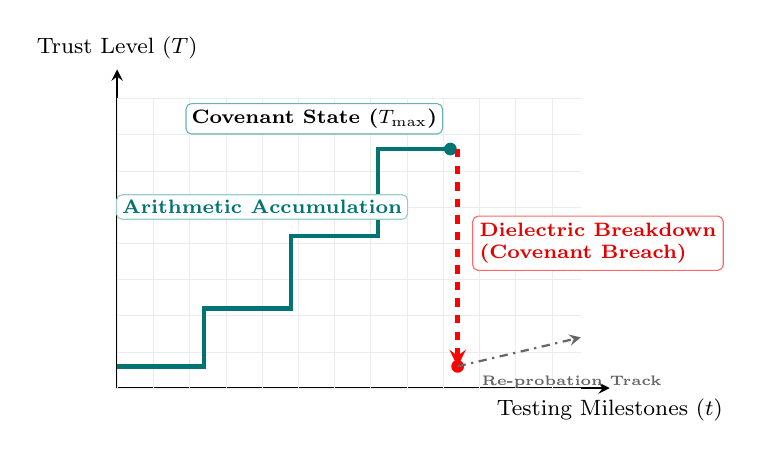
\begin{tikzpicture}[scale=0.92, >=stealth]
    \draw[->, thick] (0,0) -- (6.8,0) node[below, font=\footnotesize] {Testing Milestones ($t$)};
    \draw[->, thick] (0,0) -- (0,4.4) node[above, font=\footnotesize] {Trust Level ($T$)};
    \draw[gray!15, very thin, step=0.5] (0,0) grid (6.4,4.0);

    % Staircase
    \draw[ultra thick, teal!90!black] 
      (0,0.3) -- (1.2,0.3) 
      -- (1.2,1.1) -- (2.4,1.1) 
      -- (2.4,2.1) -- (3.6,2.1) 
      -- (3.6,3.3) -- (4.6,3.3);
    \fill[teal!90!black] (4.6,3.3) circle (2.5pt);
    \node[anchor=south east, font=\scriptsize\bfseries, fill=white, inner sep=2pt, draw=teal!60, rounded corners=2pt] at (4.5,3.5) {Covenant State ($T_{\max}$)};

    % Catastrophic collapse
    \draw[ultra thick, red, dashed, ->] (4.7,3.3) -- (4.7,0.3);
    \fill[red] (4.7,0.3) circle (2.5pt);
    \node[anchor=west, font=\scriptsize\bfseries, text=red!90!black, fill=white, inner sep=2.5pt, draw=red!60, rounded corners=2pt, align=left] at (4.9,2.0) {Dielectric Breakdown\\(Covenant Breach)};

    % Dotted re-probation
    \draw[thick, gray!80!black, dashdotted, ->] (4.7,0.3) -- (6.4,0.7);
    \node[anchor=north west, font=\tiny\bfseries, text=gray!80!black] at (4.9,0.3) {Re-probation Track};

    \node[font=\scriptsize\bfseries, text=teal!90!black, fill=white, inner sep=2pt, draw=teal!40, rounded corners=2pt] at (2.0,2.5) {Arithmetic Accumulation};
\end{tikzpicture}
\caption{\textbf{Trust Hysteresis Dynamics.} Arithmetic accumulation through testing contrasts with instantaneous geometric discharge upon defection.}
\label{fig:hysteresisbox}
\end{figure}

``Does forgiveness alter this mechanic?'' Daniel asked. ``Scripture commands forgiving seventy times seven.''

Feynman pointed his chalk directly at Daniel. ``Keep the ledger of grace separate from operational access. Forgiveness operates unilaterally. You release the debt in your heart to prevent bitterness from corroding your soul. You forgive so your standing before God remains unclouded. Trust operates bilaterally. Trust is an empirical verification of whether a counterpart handles equipment safely. You forgive the technician who dropped the radioactive isotope; you withhold the handling tongs until months of testing prove steady hands.''

\chapter{Public Decorum and Covenantal Vulnerability}

``Consider protective armor,'' Feynman said. ``Soldiers wear steel plate on the battlefield, and remove that armor when resting at home with their families.''

``The battlefield involves active hostility,'' Daniel answered.

``Exactly. The public wilderness, consisting of Tiers 0 and 1, involves competition for resources, status, and authority. That environment demands \textbf{The Power of Show}. This means decorum, professional excellence, dignified speech, and emotional self-control. You maintain clean attire, speak clearly, keep your posture upright, and keep private vulnerabilities strictly confidential.''

\begin{figure}[H]
\centering
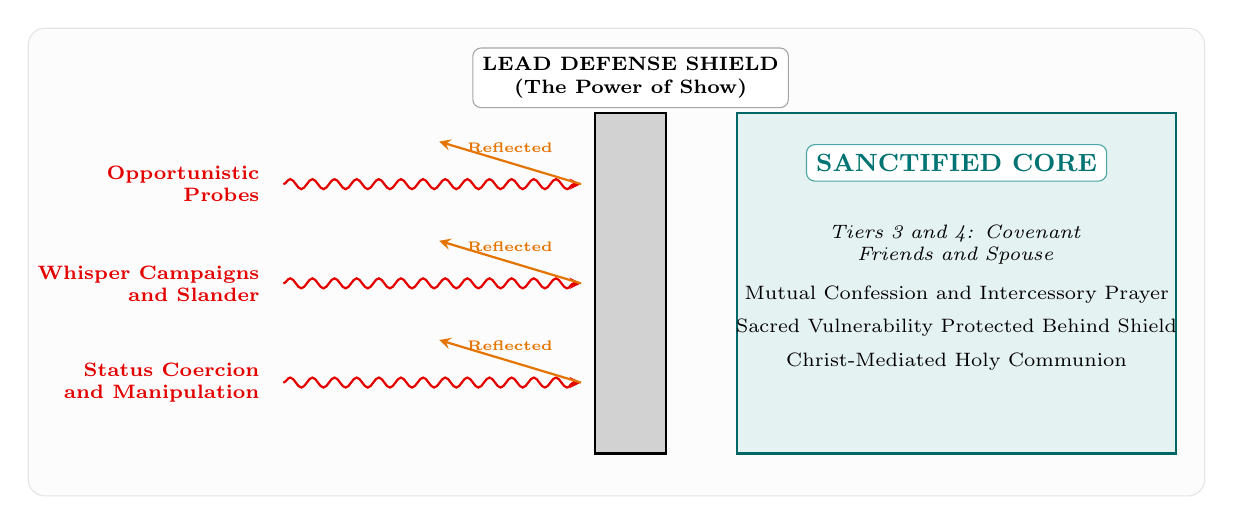
\begin{tikzpicture}[scale=0.90, >=stealth]
  % Outer Frame with generous clearance
  \draw[gray!20, fill=gray!2, rounded corners=6pt] (-4.2, -3.0) rectangle (12.4, 3.6);

  % Incoming hostile ray labels on far left
  \node[anchor=east, font=\scriptsize\bfseries, text=red!90!black, align=right] at (-0.8, 1.4) {Opportunistic\\Probes};
  \node[anchor=east, font=\scriptsize\bfseries, text=red!90!black, align=right] at (-0.8, 0.0) {Whisper Campaigns\\and Slander};
  \node[anchor=east, font=\scriptsize\bfseries, text=red!90!black, align=right] at (-0.8, -1.4) {Status Coercion\\and Manipulation};

  % Incoming wavy red rays
  \draw[->, thick, red!90!black, decorate, decoration={snake, amplitude=1.8pt, segment length=8pt}] (-0.6, 1.4) -- (3.6, 1.4);
  \draw[->, thick, red!90!black, decorate, decoration={snake, amplitude=1.8pt, segment length=8pt}] (-0.6, 0.0) -- (3.6, 0.0);
  \draw[->, thick, red!90!black, decorate, decoration={snake, amplitude=1.8pt, segment length=8pt}] (-0.6, -1.4) -- (3.6, -1.4);

  % Reflected orange rays bouncing back with labels
  \draw[->, thick, orange!90!black] (3.6, 1.4) -- (1.6, 2.0) node[midway, above, font=\tiny\bfseries, text=orange!90!black] {Reflected};
  \draw[->, thick, orange!90!black] (3.6, 0.0) -- (1.6, 0.6) node[midway, above, font=\tiny\bfseries, text=orange!90!black] {Reflected};
  \draw[->, thick, orange!90!black] (3.6, -1.4) -- (1.6, -0.8) node[midway, above, font=\tiny\bfseries, text=orange!90!black] {Reflected};

  % Lead Shield in center
  \fill[gray!35] (3.8, -2.4) rectangle (4.8, 2.4);
  \draw[thick, black] (3.8, -2.4) rectangle (4.8, 2.4);
  \node[font=\scriptsize\bfseries, fill=white, draw=gray!70, rounded corners=3pt, inner sep=3.5pt, align=center] at (4.3, 2.9) {LEAD DEFENSE SHIELD\\(The Power of Show)};

  % Clean Core Chamber on right (spacious with comfortable padding)
  \fill[teal!10] (5.8, -2.4) rectangle (12.0, 2.4);
  \draw[thick, teal!80!black] (5.8, -2.4) rectangle (12.0, 2.4);
  
  % Title banner inside the chamber at the top
  \node[font=\small\bfseries, fill=white, draw=teal!70, rounded corners=3pt, inner sep=3.5pt, text=teal!90!black] at (8.9, 1.7) {SANCTIFIED CORE};

  % Bulleted / descriptive text comfortably centered in lower section
  \node[font=\scriptsize, text width=5.6cm, align=center] at (8.9, -0.2) {
    \textit{Tiers 3 and 4: Covenant Friends and Spouse}\\[6pt]
    Mutual Confession and Intercessory Prayer\\[4pt]
    Sacred Vulnerability Protected Behind Shield\\[4pt]
    Christ-Mediated Holy Communion
  };
\end{tikzpicture}
\caption{\textbf{Radiation Shielding Mechanics.} The power of show serves as dense perimeter shielding, absorbing and reflecting external hostility so that sacred vulnerability remains secure at the core.}
\label{fig:shield}
\end{figure}

``Why?''

``Predators in any ecosystem identify vulnerable targets. Disclosing emotional wounds in a faculty meeting or corporate negotiation invites opportunistic leverage. Christ instructed the disciples: \textit{`Behold, I send you out as sheep in the midst of wolves; therefore be wise as serpents and innocent as doves'} (Matthew 10:16). The dove represents a pure heart dedicated to God. The serpent represents cognitive vigilance monitoring the social field.''

``What role remains for vulnerability?''

``Vulnerability belongs exclusively in the Holy of Holies, Tiers 3 and 4. Within a verified covenant, among comrades who have proven loyalty in shared hardship, and with a spouse before God, you lay down the armor. Vulnerability brings healing within covenant. Wearing armor in Tier 4 creates isolation. Removing armor in Tier 0 invites destruction.''

\chapter{The Social Risk Equation}

``Can we quantify social exposure?'' Daniel asked.

``Certainly,'' Feynman said, writing a formula across the board:

\begin{equation}
R_s = \frac{E \cdot H \cdot C}{I \cdot A \cdot S}
\end{equation}

\begin{blackboard}
\textbf{The Social Risk Index Parameters (Scored 1 to 10):}
\begin{itemize}
    \item $E$ (\textbf{Exposure}): The sensitivity and depth of access or private disclosures.
    \item $H$ (\textbf{Hazard Severity}): Potential damage if the counterpart defects.
    \item $C$ (\textbf{Adversarial Capacity}): Power, intelligence, and malice of the counterpart.
    \item $I$ (\textbf{Demonstrated Integrity}): Verified historical record under pressure.
    \item $A$ (\textbf{Incentive Alignment}): Degree to which their flourishing requires your flourishing.
    \item $S$ (\textbf{Structural Accountability}): Contracts, independent witnesses, and institutional checks.
\end{itemize}
\textbf{Thresholds:} $R_s \ge 3.0$ = Critical Hazard; $1.0 \le R_s < 3.0$ = Guarded Civility; $R_s < 1.0$ = Safe Covenant.
\end{blackboard}

\begin{figure}[H]
\centering
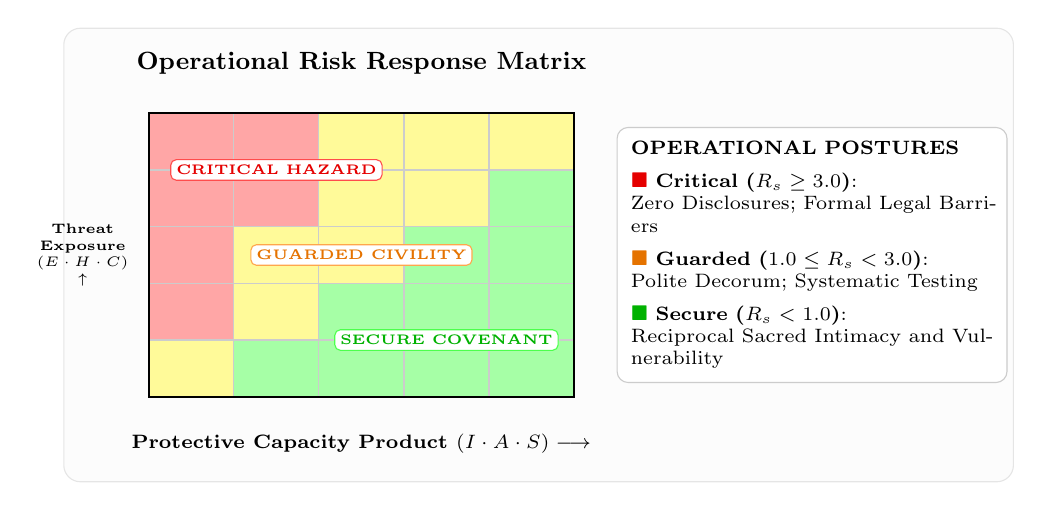
\begin{tikzpicture}[scale=0.90, >=stealth]
  % Background frame with generous margins
  \draw[gray!20, fill=gray!2, rounded corners=6pt] (-1.2, -1.2) rectangle (12.2, 5.2);

  % Top title banner
  \node[font=\small\bfseries, align=center] at (3.0, 4.7) {Operational Risk Response Matrix};

  % Heatmap matrix (5x5)
  \foreach \x in {0,1,2,3,4} {
    \foreach \y in {0,1,2,3,4} {
      \pgfmathsetmacro{\val}{(\y+1)/(\x+1)}
      \ifdim \val pt > 1.8 pt
        \fill[red!35] (\x*1.2,\y*0.8) rectangle (\x*1.2+1.2,\y*0.8+0.8);
      \else
        \ifdim \val pt > 0.8 pt
          \fill[yellow!40] (\x*1.2,\y*0.8) rectangle (\x*1.2+1.2,\y*0.8+0.8);
        \else
          \fill[green!35] (\x*1.2,\y*0.8) rectangle (\x*1.2+1.2,\y*0.8+0.8);
        \fi
      \fi
      \draw[gray!40] (\x*1.2,\y*0.8) rectangle (\x*1.2+1.2,\y*0.8+0.8);
    }
  }
  \draw[thick] (0,0) rectangle (6.0, 4.0);

  % Axis labels placed without awkward clipping
  \node[font=\scriptsize\bfseries, below=0.35cm] at (3.0, 0) {Protective Capacity Product $(I \cdot A \cdot S) \longrightarrow$};
  \node[font=\tiny\bfseries, align=center, anchor=east] at (-0.15, 2.0) {Threat\\Exposure\\$(E \cdot H \cdot C)$\\$\uparrow$};

  % Clean zone watermarks inside heatmap (properly centered)
  \node[font=\tiny\bfseries, text=red!90!black, fill=white, draw=red!70, rounded corners=2pt, inner sep=2pt] at (1.8, 3.2) {CRITICAL HAZARD};
  \node[font=\tiny\bfseries, text=orange!90!black, fill=white, draw=orange!70, rounded corners=2pt, inner sep=2pt] at (3.0, 2.0) {GUARDED CIVILITY};
  \node[font=\tiny\bfseries, text=green!70!black, fill=white, draw=green!70, rounded corners=2pt, inner sep=2pt] at (4.2, 0.8) {SECURE COVENANT};

  % Legend card on right (wide enough to prevent wrapping awkward fragments)
  \node[anchor=west, font=\scriptsize, fill=white, draw=gray!40, rounded corners=4pt, inner sep=5pt, text width=4.6cm, align=left] at (6.6, 2.0) {
    \textbf{OPERATIONAL POSTURES}\\[4pt]
    \textcolor{red!90!black}{$\blacksquare$} \textbf{Critical ($R_s \ge 3.0$)}:\\
    Zero Disclosures; Formal Legal Barriers\\[4pt]
    \textcolor{orange!90!black}{$\blacksquare$} \textbf{Guarded ($1.0 \le R_s < 3.0$)}:\\
    Polite Decorum; Systematic Testing\\[4pt]
    \textcolor{green!70!black}{$\blacksquare$} \textbf{Secure ($R_s < 1.0$)}:\\
    Reciprocal Sacred Intimacy and Vulnerability
  };
\end{tikzpicture}
\caption{\textbf{Social Risk Heatmap.} Operational postures segment into Critical Hazard, Guarded Civility, and Secure Covenant based on parameter quotients.}
\label{fig:heatmap}
\end{figure}

\chapter{Homework Problem Sets and Solutions}

\section{Problem Set 1}

\paragraph{Problem 1.1: The Rapid Confidant}
A newly hired researcher, Kevin, joins Daniel's laboratory. Within two days, Kevin shares detailed accounts of his former supervisor's perceived incompetence, discloses confidential salary information of former colleagues, and invites Daniel to share private complaints regarding the department chair.
\begin{enumerate}
    \item Evaluate Kevin across the Six Empirical Observation Vectors.
    \item Calculate the estimated Social Risk Index ($R_s$) if Daniel discloses lab funding vulnerabilities ($E=8$, $H=8$).
    \item Formulate the operational response using St.~Aelred's probation principles.
\end{enumerate}

\begin{figure}[H]
\centering
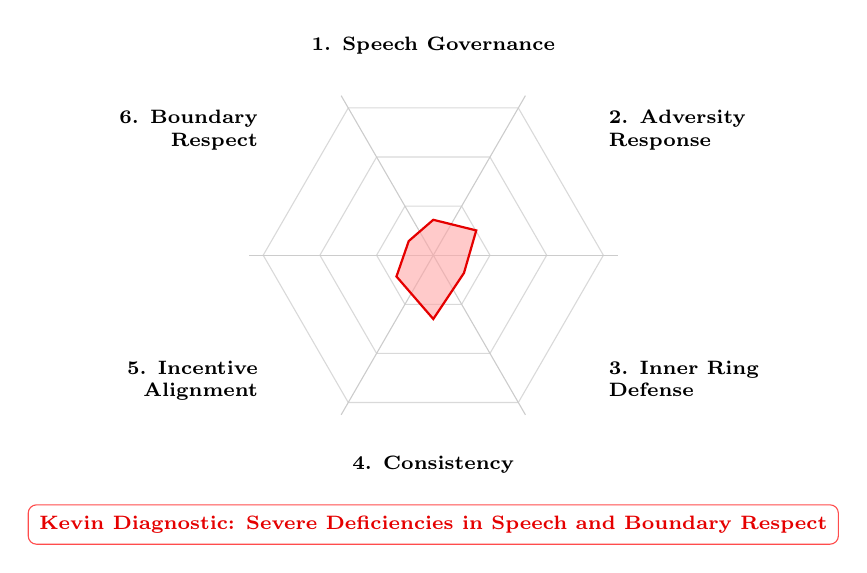
\begin{tikzpicture}[scale=0.90, >=stealth]
  % Hexagonal web
  \foreach \r in {0.8, 1.6, 2.4} {
    \draw[gray!30, thin] (0:\r) -- (60:\r) -- (120:\r) -- (180:\r) -- (240:\r) -- (300:\r) -- cycle;
  }
  \foreach \a in {0,60,120,180,240,300} {
    \draw[gray!40, thin] (0,0) -- (\a:2.6);
  }

  % Kevin polygon (defective profile)
  \fill[red!35, opacity=0.6] (90:0.5) -- (30:0.7) -- (330:0.5) -- (270:0.9) -- (210:0.6) -- (150:0.4) -- cycle;
  \draw[thick, red!90!black] (90:0.5) -- (30:0.7) -- (330:0.5) -- (270:0.9) -- (210:0.6) -- (150:0.4) -- cycle;

  % Non-overlapping labels positioned safely outside
  \node[anchor=south, font=\scriptsize\bfseries] at (90:2.7) {1. Speech Governance};
  \node[anchor=south west, font=\scriptsize\bfseries, align=left] at (30:2.7) {2. Adversity\\Response};
  \node[anchor=north west, font=\scriptsize\bfseries, align=left] at (330:2.7) {3. Inner Ring\\Defense};
  \node[anchor=north, font=\scriptsize\bfseries] at (270:2.7) {4. Consistency};
  \node[anchor=north east, font=\scriptsize\bfseries, align=right] at (210:2.7) {5. Incentive\\Alignment};
  \node[anchor=south east, font=\scriptsize\bfseries, align=right] at (150:2.7) {6. Boundary\\Respect};

  % Diagnostic callout badge with generous clearance below 4. Consistency
  \node[font=\scriptsize\bfseries, text=red!90!black, fill=white, draw=red!70, rounded corners=3pt, inner sep=4pt] at (0,-3.8) {Kevin Diagnostic: Severe Deficiencies in Speech and Boundary Respect};
\end{tikzpicture}
\caption{\textbf{Diagnostic Radar Evaluation.} Kevin displays critical deficiencies in speech governance and boundary respect.}
\label{fig:kevinradar}
\end{figure}

\begin{blackboard}
\textbf{Solution to Problem 1.1:}
\begin{enumerate}
    \item \textit{Vector Analysis}: Kevin fails Vector 1 (Speech Governance) completely. Disclosing third-party confidences caps integrity at $I \le 2$. He exhibits Vector 3 (Inner Ring Craving), using illicit secrets to manufacture an artificial in-group.
    \item \textit{Calculation}: Let $E = 8$, $H = 8$, $C = 6$. For the denominator: $I = 2$, $A = 2$ (Kevin gains status by trading gossip), $S = 2$ (casual conversation lacks contractual protection).
    \[
    R_s = \frac{8 \times 8 \times 6}{2 \times 2 \times 2} = \frac{384}{8} = 48.0
    \]
    Because $R_s = 48.0 \gg 3.0$, this interaction sits in the critical hazard zone.
    \item \textit{Protocol}: Deploy the Power of Show. Maintain polite affability (\textit{amicitia}), speak well of the department, direct conversation toward technical physics, and keep private vulnerabilities strictly confidential.
\end{enumerate}
\end{blackboard}

\section{Problem Set 2}

\paragraph{Problem 2.1: St.~Aelred's Probation Protocol}
Design a three-stage testing sequence to evaluate whether an associate qualifies for advancement from Tier 1 to Tier 2.

\begin{blackboard}
\textbf{Solution to Problem 2.1:}
\begin{enumerate}
    \item \textbf{Discretion Probe (\textit{Discretio})}: Confide an innocuous, harmless personal plan with an explicit privacy request: \textit{``I am drafting a paper for the spring symposium; please keep this between us until the draft is complete.''} Monitor whether rumors surface over three weeks.
    \item \textbf{Reliability Probe (\textit{Fides})}: Request review of a brief technical appendix with a concrete deadline. Observe punctual completion and treatment of materials.
    \item \textbf{Friction Probe (\textit{Patientia})}: Express a polite, well-reasoned dissent regarding an opinion held by the candidate. Observe whether they respond with rational engagement or defensive withdrawal and resentment.
\end{enumerate}
\end{blackboard}

\chapter{Examinations and Solutions}

\section{Midterm Examination}

\paragraph{Question 1: Theological Hermeneutics}
Explain the operational difference between \textit{Agape} (unconditional love) and \textit{Fides} (interpersonal trust) using John 2:23-25 and Matthew 7:6.

\begin{blackboard}
\textbf{Midterm Solution 1:}
\textit{Agape} is a unilateral theological virtue commanded toward all people, including adversaries. It wills the objective good of the other person and seeks their ultimate flourishing regardless of their merit. \textit{Fides} (trust) is a relational evaluation based on verified moral and functional character. In John 2:23-25, Christ exemplified \textit{agape} by ministering to the crowds while withholding personal entrustment (\textit{episteuen}) because He understood human fallenness. Conflating \textit{agape} with \textit{fides} leads people to view boundaries as uncharitable, granting untrustworthy actors access to vulnerable assets and causing structural exploitation.
\end{blackboard}

\section{Final Comprehensive Examination}

\paragraph{Case Study: The Department Crisis}
Professor Vance approached Daniel during the spring semester. Vance offered Daniel co-authorship on a major research grant. However, Vance required that Daniel avoid consulting the laboratory director, Dr.~Hastings, claiming Hastings would claim the credit. Vance changes student assistants annually, praises Daniel as the only brilliant student in the cohort, and requests that Daniel sign the budget authorization before the final line items are completed.
\begin{enumerate}
    \item Calculate the Social Risk Index ($R_s$) for signing the authorization.
    \item Identify the manipulative tactics employed by Vance using C.S.~Lewis's \textit{The Inner Ring} and Aquinas's analysis of vices.
    \item Draft the exact response Daniel must deliver to Vance using the Operational Playbook.
\end{enumerate}

\begin{figure}[H]
\centering
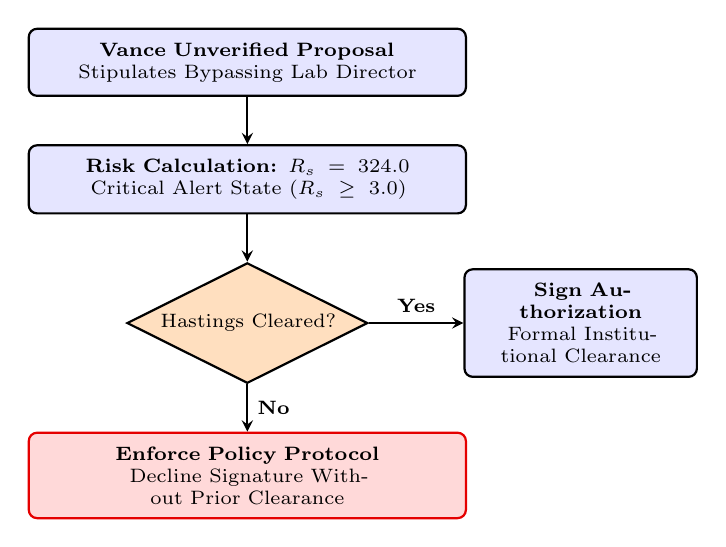
\begin{tikzpicture}[auto, >=stealth,
    block/.style={rectangle, rounded corners=3pt, draw=black, thick, fill=blue!10, text width=5.2cm, text centered, font=\scriptsize, inner sep=5pt},
    decision/.style={diamond, draw=black, thick, fill=orange!25, text width=2.2cm, text centered, font=\scriptsize, inner sep=2pt, aspect=2},
    stopblock/.style={rectangle, rounded corners=3pt, draw=red!90!black, thick, fill=red!15, text width=5.2cm, text centered, font=\scriptsize, inner sep=5pt}]

    \node[block] (trigger) {\textbf{Vance Unverified Proposal}\\Stipulates Bypassing Lab Director};
    \node[block, below=0.6cm of trigger] (eval) {\textbf{Risk Calculation: $R_s = 324.0$}\\Critical Alert State ($R_s \ge 3.0$)};
    \node[decision, below=0.6cm of eval] (d1) {Hastings Cleared?};
    \node[block, right=1.2cm of d1, text width=2.6cm] (sign) {\textbf{Sign Authorization}\\Formal Institutional Clearance};
    \node[stopblock, below=0.6cm of d1] (decline) {\textbf{Enforce Policy Protocol}\\Decline Signature Without Prior Clearance};

    \draw[->, thick] (trigger) -- (eval);
    \draw[->, thick] (eval) -- (d1);
    \draw[->, thick] (d1) -- node[above, font=\scriptsize\bfseries] {Yes} (sign);
    \draw[->, thick] (d1) -- node[right, font=\scriptsize\bfseries] {No} (decline);
\end{tikzpicture}
\caption{\textbf{Operational Decision Protocol for Vance Case Study.} Formal audit gates prevent asymmetric liability transfer.}
\label{fig:decisiontree}
\end{figure}

\begin{blackboard}
\textbf{Final Exam Solutions:}
\begin{enumerate}
    \item \textit{Risk Calculation}: $E=9, H=9, C=8$. For the denominator: $I=2$ (annual assistant turnover), $A=1$ (asymmetric risk: Vance secures credit, Daniel assumes legal liability), $S=1$ (bypassing Dr.~Hastings eliminates institutional oversight).
    \[
    R_s = \frac{9 \times 9 \times 8}{2 \times 1 \times 1} = \frac{648}{2} = 324.0 \quad (\text{Critical Hazard Zone})
    \]
    \item \textit{Tactical Analysis}: Vance utilizes the Inner Ring mechanism by flattering Daniel's ego (the only brilliant student) and offering exclusive status while excluding legitimate authority. He employs \textit{adulatio} (flattery, ST II-II, q. 115) and attempts to bypass verification, a recognized predatory tactic.
    \item \textit{Scripted Response}:
    \begin{quote}
    ``Thank you for the opportunity, Professor Vance. Institutional protocol requires that all grant budget authorizations undergo formal review by Dr.~Hastings as laboratory director prior to signature. I will gladly sign once Dr.~Hastings has reviewed the completed line items and granted formal clearance.''
    \end{quote}
\end{enumerate}
\end{blackboard}

\end{document}
